\documentclass[11pt]{article}
\usepackage[letterpaper,margin=1in]{geometry}
\usepackage[T1]{fontenc}
\usepackage{mathptmx}
\usepackage{amsmath,amssymb}
\usepackage{graphicx}
\usepackage{booktabs}
\usepackage[font=small,labelfont=bf]{caption}
\usepackage[numbers,sort&compress]{natbib}
\usepackage{xcolor}
\usepackage{microtype}
\usepackage{authblk}
\usepackage[colorlinks=true,linkcolor=blue!50!black,citecolor=blue!50!black,urlcolor=blue!50!black]{hyperref}
\setlength{\emergencystretch}{3em}
\renewcommand{\baselinestretch}{1.12}

\title{Dipole matrix elements of nonparabolic quantum-well states: the two-band norm, and a truncation artefact of L\"owdin orthonormalization}
\author{Gracen Ownby}
\affil{University of Oklahoma, Norman, Oklahoma, USA}
\date{\small 14 October 2026}

\begin{document}
\maketitle

\begin{abstract}
Intersubband dipole matrix elements are routinely computed from the one-band Schr\"odinger equation with an energy-dependent effective mass. Its eigenstates belong to different Hamiltonians and are not orthonormal in the ordinary inner product; they are orthonormal only as two-component states of the two-band Kane model from which the energy-dependent mass derives. We compare the common remedies against the two-band dipoles for three InGaAs/InAlAs structures (a double well, a biased triple well and a single well) in boxes of 100--400~\AA\ of barrier. Without orthogonalization the dipoles are off by 2--6\% for strong transitions and by up to 25\% for weak ones, and they depend on the coordinate origin. Two errors are at work. The one-band norm misses the light-hole weight of each state, which alone makes the dipole of a single well 5\% too large even though its two states are orthogonal by parity; Gram--Schmidt and L\"owdin orthonormalization of the bound states cannot correct it. Symmetric (L\"owdin) orthonormalization of the bound states alone adds a second error: the topmost bound state cannot be orthogonalized against the states left out, and its dipoles come out 5--11\% wrong when it is well bound and 37\% wrong when it is close to the barrier edge, independently of the box size. A first-order expansion reproduces this error to 0.4 percentage points and shows that it comes entirely from the missing partners. Orthonormalizing the bound states together with all box states within 0.5~eV above the topmost one brings every dipole within 1.2\% of the two-band value (0.8\% for boxes of 150~\AA\ or more), and peak second-order susceptibilities within 1.1\%; a fixed small number of extra states does not, and can make the error larger. The two-band norm itself removes both errors at no cost and needs no extra states; we recommend it.
\end{abstract}

\section{Introduction}
Most calculations of intersubband (ISB) absorption, quantum-cascade transport and ISB nonlinear optics in narrow-gap quantum wells use a one-band envelope equation in which the effective mass depends on energy \cite{Nelson1987,Ekenberg1989,Sirtori1994,JirauschekKubis2014},
\begin{equation}
-\frac{d}{dz}\frac{\hslash^2}{2m(E,z)}\frac{d\psi}{dz}+V(z)\psi=E\psi,\qquad m(E,z)=m^*(z)\left[1+\frac{E-V(z)}{E_g(z)}\right].
\label{eq:H}
\end{equation}
The eigenproblem is nonlinear in $E$: each eigenvalue belongs to its own Hamiltonian $H(E)$, so eigenstates of different energy are not orthogonal in the ordinary inner product \cite{JirauschekKubis2014,Jonasson2016,Mohamed2024}. The equation derives from a two-band Kane model, in which each state has a light-particle component
\begin{equation}
\phi_n(z)=\sqrt{\frac{\hslash^2E_g}{2m^*}}\,\frac{\psi_n'(z)}{E_n-V(z)+E_g},
\label{eq:phi}
\end{equation}
and the two-component states are orthogonal, $\int(\psi_m\psi_n+\phi_m\phi_n)\,dz=N_n\delta_{mn}$ \cite{Sirtori1994,Mohamed2024}; the same norm follows from the general rule for energy-dependent Hamiltonians, $\langle\psi|1-\partial H/\partial E|\psi\rangle$ \cite{Formanek2004}. Codes handle the overlap in different ways. Some use the two-band (or three-band) norm, some avoid the energy-dependent mass altogether \cite{Jonasson2016}, and many ignore the overlap or orthonormalize the bound states, by Gram--Schmidt or by L\"owdin's symmetric orthonormalization \cite{Lowdin1950}, which changes the states least in the least-squares sense \cite{CarlsonKeller1957}. The differences are of the order of $(E-V)/E_g$, a few per cent, and are often regarded as negligible.

In the course of auditing a set of calculations of ISB second-order nonlinearities we found that L\"owdin orthonormalization of the bound states alone gave one structure a second-order susceptibility 8\% too large, an error that depended on how many states happened to be bound and that earlier checks in a smaller box had hidden. To our knowledge this artefact has not been reported. Here we quantify the errors of the common procedures against the two-band dipoles, identify their two sources, and give a simple rule.

\section{Method}
We solve Eq.~\eqref{eq:H} self-consistently (Hartree) for In$_{0.53}$Ga$_{0.47}$As wells ($m^*=0.043\,m_0$, $E_g=0.75$~eV) and In$_{0.52}$Al$_{0.48}$As barriers ($0.075\,m_0$, 1.45~eV, offset 0.52~eV) with $5\times10^{11}$~cm$^{-2}$ electrons at 300~K, on a 0.5~\AA\ grid with hard walls at the ends of a barrier padding of 100--400~\AA\ (half on each side), using qwkit \cite{qwkit}. The structures are a 64/10/29~\AA\ asymmetric double well (three or four bound states), a 58/14/34/14/58~\AA\ triple well at 55~kV/cm (five), and a 60~\AA\ single well (two, or three in the 100~\AA\ box). States with at least 80\% of their probability within 25~\AA\ of the wells count as bound; the box states above them form a discrete quasi-continuum whose density grows with the box. We compare, against the two-band dipoles $z^K_{mn}=\int(\psi_mz\psi_n+\phi_mz\phi_n)\,dz/\sqrt{N_mN_n}$ (whose two-band overlaps are below $4\times10^{-5}$ here):
\begin{itemize}
\item \emph{raw}: normalized one-band states without orthogonalization;
\item \emph{GS}: Gram--Schmidt of the bound states from the lowest up;
\item \emph{L-bound}: L\"owdin orthonormalization of the bound states, $\tilde\Psi=\Psi S^{-1/2}$ with $S=\Psi^T\Psi$;
\item \emph{L-buffer}: L\"owdin orthonormalization of the bound states together with the next $n$ box states ($n=1$--20), or with all box states up to $\Delta E=0.1$--1~eV above the topmost bound state, then truncated to the bound states.
\end{itemize}
We report relative errors of all allowed dipoles $z_{mn}$ between the lowest four bound states and of the peak second-order susceptibility for second-harmonic generation through the lowest three states (linewidth 10~meV).

\section{Results}
Figure~\ref{fig:err} shows the largest dipole error of each procedure against the box size, and Table~\ref{tab:err} lists the largest errors.

\emph{Raw states.} The one-band overlaps reach 0.025--0.04 between bound states. Without orthogonalization the strong dipoles $z_{12}$, $z_{23}$ are off by 2--3\% and $z_{13}$ by 5--6\%; weak transitions are worse ($z_{24}$ of the triple well $-21$ to $-25$\%, $z_{14}$ of the double well $+108$\% in the 100~\AA\ box). Raw dipoles also depend on the origin of $z$, because $\langle m|z+a|n\rangle=z_{mn}+aS_{mn}$: moving the origin by 100~\AA\ changes the error of $z_{12}$ of the double well from $+2$ to $+15$\% and that of $z_{13}$ from $+6$ to $-14$\%. The peak susceptibility of the double well is 10\% too large.

\emph{Norm.} The single well isolates the norm. Its two bound states have opposite parity and are exactly orthogonal, yet $z_{12}$ is 5.0\% too large in every box, with or without Gram--Schmidt or L\"owdin orthonormalization of the bound states, which do nothing here. The one-band norm $\int\psi^2dz=1$ omits the light-particle weight $\int\phi^2dz$ of Eq.~\eqref{eq:phi}, which is larger for the excited state, and the light-particle components contribute their own dipole. Neither correction can come from orthogonalizing the bound states among themselves. Gram--Schmidt leaves errors of 2--5\% in all structures (18\% for the weak $z_{14}$).

\emph{Truncation.} L\"owdin orthonormalization of the bound states corrects the dipoles among the lower states of the double and triple wells to within 0.8\% but not those of the topmost bound state: $z_{13}$ of the double well (three bound states) is 6.7--6.8\% too large in all boxes of 150~\AA\ or more, against 5.8\% without orthogonalization; $z_{14}$ in the 100~\AA\ box, where a fourth state is barely bound, is 37\% too large; $z_{14}$ and $z_{24}$ of the triple well are off by 5.3\% and 9--11\%. The peak susceptibility of the double well comes out 8.8\% too large. Expanding $S^{-1/2}=1-\tfrac12D+O(D^2)$ with $D=S-1$,
\begin{equation}
\tilde z_{mn}\approx z_{mn}-\tfrac12\sum_{k\in\mathcal B}\left(S_{mk}z_{kn}+z_{mk}S_{kn}\right),
\end{equation}
where $\mathcal B$ is the set orthonormalized, reproduces the L-bound errors to 0.4 percentage points in all cases. For a state in the middle of the set, its overlaps with the states above and below enter with their dipoles, and the corrections largely restore what the two-band norm would give. For the topmost state, the partners above it are missing from $\mathcal B$; their contributions, $\tfrac12S_{t,t+1}z_{t+1,n}$ and so on, are never subtracted. Because the dipoles to the next state up are the largest, the omission is not small. The error does not shrink with a larger box, because it is set by the bound states, and it changes abruptly when a state becomes bound or unbound with a change of structure, field or density.

\emph{Buffers.} Including box states above the bound ones restores the missing partners. A buffer of all states within 0.5~eV above the topmost bound state brings every allowed dipole within 1.2\% of the two-band value in all structures and boxes (within 0.8\% for boxes of 150~\AA\ or more) and the peak susceptibility within 1.1\%; 1~eV gives 0.4--0.6\% except for the 100~\AA\ box. A buffer of a fixed number of states is unreliable: the energy it spans shrinks as the box grows, and with two extra states the error of $z_{13}$ of the double well grows from 0.6 to 6.6\% between 100 and 400~\AA\ of padding, while $z_{24}$ of the triple well is off by up to 17\%, worse than with no buffer. Ten extra states suffice in the boxes studied (at most 1.5\%), because they span more than 0.5~eV there. That the buffered L\"owdin dipoles also absorb the norm error of the single well (within 0.7\% for padding of 150~\AA\ or more) shows that the overlaps of a bound state with the quasi-continuum carry its light-particle weight; we have not found a proof that the agreement becomes exact as the buffer grows, and in our calculations it saturates at a few tenths of a per cent.

\begin{figure}[t]
\centering
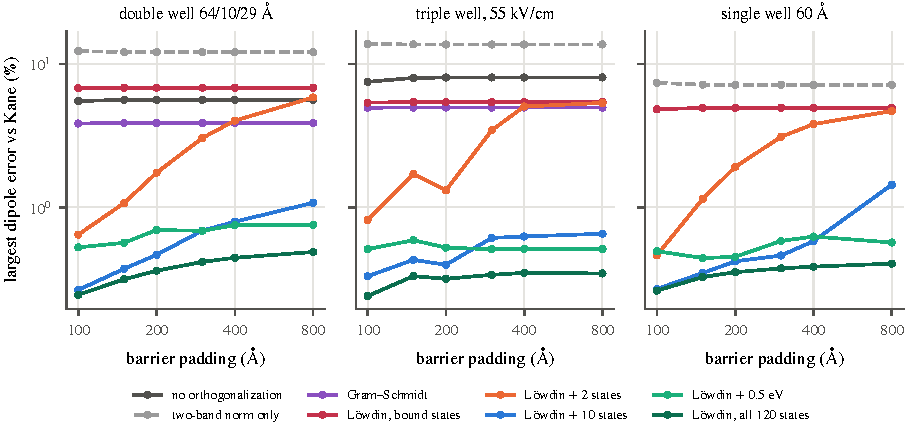
\includegraphics[width=\textwidth]{figures/fig1_errors.pdf}
\caption{Largest relative error of the allowed dipoles between the lowest four bound states, against the two-band Kane dipoles, as a function of the barrier padding (box size), for six procedures. Errors below 0.05\% are drawn at 0.05\%.}
\label{fig:err}
\end{figure}

\begin{table}[t]
\centering
\small
\caption{Largest relative dipole error (\%) against the two-band dipoles over all allowed transitions among the lowest four bound states, for barrier paddings of 150--400~\AA\ (100--400~\AA\ in parentheses where different).}
\label{tab:err}
\begin{tabular}{lccc}
\toprule
Procedure & double well & triple well, 55 kV/cm & single well \\
\midrule
raw & 5.8 (108) & 25 & 5.0 (10) \\
Gram--Schmidt & 3.7 (18) & 4.7 & 5.0 \\
L\"owdin, bound states only & 6.8 (37) & 11 & 5.0 (7.7) \\
L\"owdin + 2 states & 6.6 & 17 & 4.9 \\
L\"owdin + 10 states & 0.8 (1.5) & 1.0 & 0.7 \\
L\"owdin + 0.5 eV & 0.8 (1.2) & 0.6 & 0.7 \\
L\"owdin + 1 eV & 0.6 (1.6) & 0.4 & 0.5 \\
\bottomrule
\end{tabular}
\end{table}

\section{Recommendation}
The two-band norm is exact within the model, costs one derivative per state, and needs no states beyond those of interest: compute $\phi_n$ from Eq.~\eqref{eq:phi} and use $z^K_{mn}$, as Mohamed \emph{et al.} also recommend for quantum-cascade levels \cite{Mohamed2024}. Its orthogonality, to a few $10^{-5}$ on a 0.5~\AA\ grid here, is a useful check of the eigensolver. If a code must orthonormalize one-band states, it should do so over the bound states and all box states within at least 0.5~eV above them (or test the result against a larger buffer), never over the bound states alone, and should not use a fixed small number of extra states. Raw one-band dipoles depend on the coordinate origin and should not be used for weak transitions.

The errors matter most where the topmost bound state takes part: second-order nonlinearities of double-resonance designs, where the third state is often the topmost bound one, and weak transitions that set selection-rule-sensitive figures of merit. For the double well studied here, the susceptibility error of L\"owdin over the bound states (8.8\%) exceeds typical design tolerances, and it varies with the box and with the number of bound states, so that design optimizations or uncertainty analyses that cross the binding of a state see a spurious jump.

\section{Conclusion}
One-band dipoles of nonparabolic quantum-well states carry two distinct errors: a norm error of a few per cent that orthogonalization among bound states cannot remove, and, when L\"owdin orthonormalization is restricted to the bound states, a truncation error of 5--40\% in the dipoles of the topmost bound state. The two-band norm removes both exactly; a L\"owdin buffer of 0.5~eV of box states removes them to about 1\%. The calculations use qwkit \cite{qwkit}, whose versions up to 0.6.0 had the truncation error and which since 0.6.1 buffers its orthonormalization and offers the two-band dipoles.

\bibliographystyle{unsrtnat}
\bibliography{refs}
\end{document}
